\documentclass[a4paper,10pt]{article}
\usepackage[utf8]{inputenc}
\usepackage{hyperref}
\usepackage{mathtools}
\usepackage{graphicx}
\usepackage[labelfont=bf]{caption}
%opening
\author{
  Oluwasanmi Koyejo\\
  Srinivasan Sivaramachandran
  \and
  Pradeep Ravikumar\\
  Russell A. Poldrack
}
\title{Combining fMRI, DTI and Behavioral Information : A Novel Modeling Approach}

\begin{document}

\maketitle



\section{Introduction}
This write-up presents the approach discussed towards simulating a working model towards generating fMRI, DTI and behavioral information. The code and clear instructions are available at \url{http://www.github.com/srini21/fmri-sim} .

\section{Modeling methodology}
The integral part of the approach is that the fMRI and the DTI share the same basic structure but the strength of the connections i.e the weight modified by the behavioral data varies. The basic steps discussed are explained as follows: 

\subsection{Graph Topology}
The first step involves determining the graph topology. The discussions involved using either ring topology or star topology to represent the brain structure. It was finalized to align as close as possible to the simulations done by Smith et  al \cite{smith} is shown in the figure 1.  
\begin{figure}[b]
\center
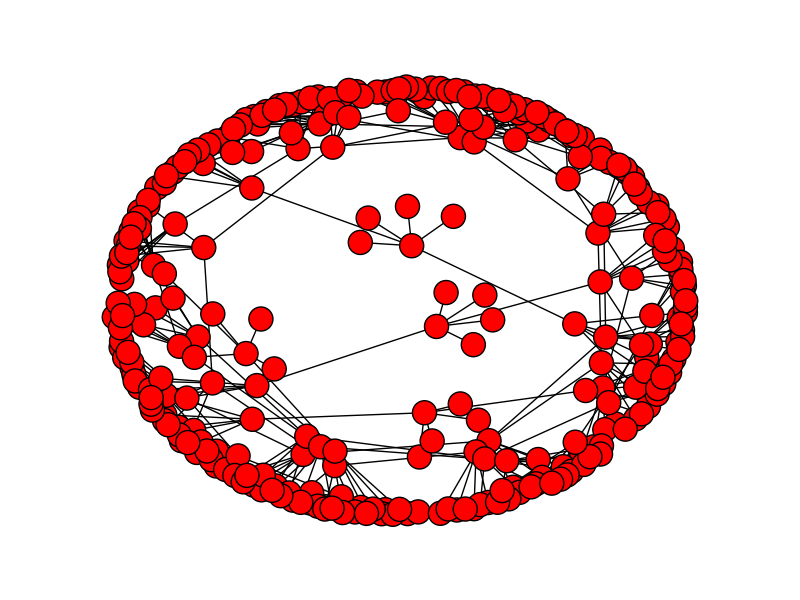
\includegraphics[scale=0.3]{graphRep.png}

\caption{Representation of the graph structure with star topology. Number of nodes = 300, number of sub-nodes = 5}

\end{figure}
$\mathcal{G}_{s,t} \in \Re^{n*n}$ represents the adjacency matrix of the above mentioned graph where n represents the number of nodes in the brain.
\subsection{Age}
As an outcome of our meeting dated July 22, we decided that the age of the subjects ranged from 7 to 22. Hence, $\forall individual$, we generate $\{A_{p}\}_{p=1}^{n}$ = $\{a_{1},a_{2}, .. a_{n}\}$ where n is the number of age samples for every individual.
\subsection{Behavioral Information}
$b_{i} \in \Re^{d}$ represents the behavioral information at age $i$ where $d$ represents the number of behavioral features collected from every individual. $\exists b_{0} \forall$ individuals drawn from $\mathcal{N}(0,1)$ . This $b_{0}$ is used to generate a time series of behavioral information $\forall ages$ for that person using the formula
\begin{align*}
b_{a+1}=\mathcal{F}_{p}b_{a} + noise
\end{align*}
where $\mathcal{F} \in \Re^{d*d}$ is also drawn from $\mathcal{N}(0,1) \forall person$.  

In order to preserve the effects of age, the behavior vector used for computation will be $\mathcal{X} \in \Re^{d+2} = \begin{bmatrix}
      b_{i} \\
      i \\
      1
    \end{bmatrix}$ where $b_{i} \in \Re^{d}$ represents the computed behavior vector for age $i$ . 
\subsection{fMRI Weights and DTI weights}
$\mathcal{W}^{d}$ and $\mathcal{W}^{f} \in \Re^{n*n*(d+2)}$  represent the weights associated with the DTI and the fMRI data respectively where n represents the number of nodes in the graph and d represents the behavioral features. The weight matrices are generated so that they preserve block sparsity i.e $\mathcal{W}^{f}_{s,t},{W}^{d}_{s,t}=0$ if $\mathcal{G}_{s,t}=0$
\subsection{$\theta_{s,t}$ for fMRI and DTI}
The formula for generating $\theta^{f}$ and $\theta^{d}$ are shown below :
\begin{align*}
\forall _{s,t} \hspace{10pt} \theta^{f}_{s,t}(b,a)= (\mathcal{W}^f_{s,t})^T * \mathcal{X} \\
\forall _{s,t} \hspace{10pt} \theta^{d}_{s,t}(b,a)= (\mathcal{W}^d_{s,t})^T * \mathcal{X} \\
\end{align*}
where $\mathcal{X} =
\begin{bmatrix}
      b_{i} \\
      i \\
      1
    \end{bmatrix} \in \Re^{d+2}$ and $\theta \in \Re^{n*n*d+2}$
\subsection{Sampling $\mathcal{Y}$}
We finally sample $\mathcal{Y}$ where $\mathcal{Y}^{f}$,$\mathcal{Y}^{d}$ $\in \Re^{d}$ as follows :
\begin{align*}
\mathcal{Y}^{f} \sim \mathcal{P}(\mathcal{Y};\theta^{f})\\
\mathcal{Y}^{f} \sim \mathcal{P}(\mathcal{Y};\theta^{f})
\end{align*}
\section{Further Steps}
Next steps involve discussing the fitting procedure and other alternatives during our meeting on 7/30. 
\begin{thebibliography}{99}
    \bibitem{smith} Stephen M. Smith, Karla L. Miller, Gholamreza Salimi-Khorshidi, Matthew Webster, Christian F. Beckmann, Thomas E. Nichols, Joseph D. Ramsey, Mark W. Woolrich, Network modelling methods for FMRI, NeuroImage, Volume 54, Issue 2, 15 January 2011, Pages 875-891, ISSN 1053-8119, \url{http://dx.doi.org/10.1016/j.neuroimage.2010.08.063}

    
\end{thebibliography}

\end{document}
